% =============================================================
%  Fervo Cape Station Phase 2 — PSLF Model Representation
%  Uses the shared American Terawatt report style.
%  Compile:  pdflatex fervo.tex   (run twice for ToC / references)
%  The dynamic-model parameter tables in tables/ are generated from the
%  .dyd file in references/ by  python3 gen_tables.py
% =============================================================
\documentclass[11pt,a4paper]{article}

% Shared style lives in the repo-level template folder
\usepackage[corporate]{../../template/attemplate}
\usepackage{pgfplots}
\pgfplotsset{compat=1.18}
\usepackage{placeins}
\usepackage{url}
\def\UrlBreaks{\do\_\do\.\do\-\do\ \do\a\do\b\do\c\do\d\do\e\do\f\do\g\do\h\do\i\do\j\do\k\do\l\do\m\do\n\do\o\do\p\do\q\do\r\do\s\do\t\do\u\do\v\do\w\do\x\do\y\do\z\do\0\do\1\do\2\do\3\do\4\do\5\do\6\do\7\do\8\do\9\do\A\do\B\do\C\do\D\do\E\do\F\do\G\do\H\do\I\do\J\do\K\do\L\do\M\do\N\do\O\do\P\do\Q\do\R\do\S\do\T\do\U\do\V\do\W\do\X\do\Y\do\Z}

% TikZ libraries used by the one-line and block diagrams
\usetikzlibrary{arrows.meta,positioning,calc,shapes.geometric,fit}

% Block-diagram styles shared by figures/*.tex
\tikzset{
  blk/.style={draw=atFg,thick,rectangle,minimum height=9mm,minimum width=14mm,align=center,inner sep=2pt,font=\small},
  sum/.style={draw=atFg,thick,circle,minimum size=5mm,inner sep=0pt,font=\footnotesize},
  lim/.style={draw=atFg,thick,rectangle,minimum height=9mm,minimum width=10mm,align=center,font=\small},
  sig/.style={-{Latex[length=2mm]},thick,draw=atFg},
  lbl/.style={font=\footnotesize},
  bus/.style={line width=2.2pt,draw=atFg},
  node distance=6mm and 9mm,
}

% ---- Report metadata ----------------------------------------
\reporttitle{Fervo Cape Station}
\reportsubtitle{PSLF model representation --- physical network and dynamic controls}
\reportauthor{Eugen Starschich}
\reportdocnumber{ATW-REP-FERVO-001}
\reportrevision{0.1}
\reportstatus{Draft}
\reportdate{\today}
\reportconfidentiality{Confidential}

\begin{document}

\makecover

\revisionhistory{
  \revrow{0.1}{Sep. 17, 2026}{Eugen Starschich}{Initial document}
}

\newpage
\tableofcontents
\clearpage

% ---- Body ---------------------------------------------------
\section{Scope}

This document sets out the PSLF model of Fervo Cape Station Phase~2 as delivered in
the two source files listed in Section~\ref{sec:refs}: a power-flow network case
(\texttt{.epc}, PSLF version~24.3.0)~[1] and a dynamic-data file (\texttt{.dyd})~[2].
The representation is split into a \emph{physical part} --- buses, lines, transformers,
generators and loads that define the steady-state network --- and a \emph{control
part} --- the machine, excitation, governor, stabilizer and protection models that
define the dynamic behaviour of each unit.

The plant comprises nine steam-turbine generators at 13.8\,kV, arranged in pairs on
four generator buses, each pair stepped up through its own 150\,MVA generator
step-up transformer (GSU) to a 345\,kV collector bus (GEN-TIE). The collector bus
connects over a 3.0\,mile line to the point of interconnection (POI), which is
represented as an infinite bus in the dynamic data. A 3.2\,mile line from GEN-TIE to
the Phase~1 main power transformer bus (HV-MPT-P1) is included in the network case
as the tie to Phase~1.

Two families of units appear in the data. Units~4, 5 and~6 are Turboden machines
rated 76.471\,MV$\cdot$A, and units~7 through~11 are Baker Hughes machines rated
71.13\,MV$\cdot$A. The two families share the same excitation, stabilizer and
protection settings but have different machine constants and turbine capabilities.
Every parameter value in the tables of this document is transcribed from the source
files by script, so the tables can be regenerated whenever the files change.

\section{Physical network model}
\label{sec:network}

The network case contains 11 buses, 6 branches, 4 transformers, 9 generators plus the
POI swing source, and 4 loads. All equipment is assigned to area~26 (LADWP) and
zone~283 (LA~IPP). The system base is 100\,MV$\cdot$A. Figure~\ref{fig:oneline}
shows the one-line arrangement.

\begin{figure}[!ht]
\centering
\resizebox{\linewidth}{!}{%
\begin{tikzpicture}[x=1cm,y=1cm,font=\footnotesize]
  % POI
  \draw[bus] (-1.2,10) -- (1.2,10) node[right,xshift=2mm]{\textbf{1 POI} 345\,kV\quad(swing, $U_{sched}=1.0493$)};
  \draw (0,10) -- (0,8.6);
  \node[right,align=left] at (0.15,9.3) {3.0\,mi, 1590 kcmil Lapwing\\1077.7\,MV$\cdot$A};
  % GEN-TIE busbar
  \draw[bus] (-6.4,8.6) -- (6.4,8.6) node[right,xshift=2mm]{\textbf{18 GEN-TIE} 345\,kV};
  % tie to Phase 1
  \draw (-6.0,8.6) -- (-6.0,7.6) -- (-7.4,7.6);
  \draw[bus] (-7.4,7.1) -- (-7.4,8.1);
  \node[left,align=right] at (-7.5,7.6) {\textbf{2 HV-MPT-P1}\\345\,kV (Phase~1)};
  \node[above,align=center] at (-6.7,7.65) {3.2\,mi\\Lapwing};
  % four feeders
  \foreach \x/\b/\g/\len/\gsu/\u in {
      -4.5/19/17/0.60/HV-GSU-P2-1/{4, 5},
      -1.5/20/22/0.74/HV-GSU-P2-2/{6, 7},
       1.5/21/23/2.81/HV-GSU-P2-3/{8, 9},
       4.5/28/25/2.88/HV-GSU-P2-4/{10, 11}}{
    \draw (\x,8.6) -- (\x,7.0);
    \node[right,align=left] at (\x+0.08,7.85) {\len\,mi\\Waxwing};
    \draw[bus] (\x-0.8,7.0) -- (\x+0.8,7.0);
    \node[above left,align=right,yshift=-0.3mm] at (\x-0.8,7.0) {\textbf{\b}};
    \node[below,align=center] at (\x,6.95) {\gsu\\345\,kV};
    % transformer
    \draw (\x,6.35) -- (\x,5.95);
    \draw (\x,5.6) circle (0.35);
    \draw (\x,5.1) circle (0.35);
    \draw (\x,4.75) -- (\x,4.4);
    \node[right,align=left,font=\scriptsize] at (\x+0.4,5.35) {150\,MV$\cdot$A\\$X_T = 14.5\,\%$\\362/13.8\,kV};
    % gen bus
    \draw[bus] (\x-0.9,4.4) -- (\x+0.9,4.4);
    \node[above left,align=right,yshift=-0.3mm] at (\x-0.9,4.4) {\textbf{\g}};
    \node[below left,align=right,font=\scriptsize,yshift=0.3mm] at (\x-0.9,4.4) {13.8\,kV};
    % two generators
    \draw (\x-0.55,4.4) -- (\x-0.55,3.75);
    \draw (\x-0.55,3.35) circle (0.4) node{G};
    \draw (\x+0.55,4.4) -- (\x+0.55,3.75);
    \draw (\x+0.55,3.35) circle (0.4) node{G};
    % load arrow
    \draw[-{Latex[length=2mm]}] (\x,4.4) -- (\x,2.6);
    \node[below,align=center] at (\x,2.55) {aux\\load};
    \node[below,align=center] at (\x,1.9) {units \u};
  }
\end{tikzpicture}
}
\caption{One-line diagram of the Phase~2 network case. Bus numbers are those of the \texttt{.epc} file; line lengths and conductor types are taken from the branch records.}
\label{fig:oneline}
\end{figure}

\subsection{Buses}

Table~\ref{tab:bus} lists the buses. Bus~1 is the swing bus (PSLF type~0) with a
scheduled voltage of 1.0493\,pu; the four generator buses are voltage-controlled
(type~2) at 1.00\,pu, regulating their own terminals; the remaining 345\,kV buses are
load buses (type~1). Every bus carries the same 0.95--1.05\,pu voltage band.

\begin{table}[!ht]
\centering
\begin{tabularx}{\linewidth}{@{}r l r c r X@{}}
\toprule
\multicolumn{1}{c}{\textbf{No.}} & \textbf{Name} & \multicolumn{1}{c}{\textbf{kV}} & \multicolumn{1}{c}{\textbf{Type}} & \multicolumn{1}{c}{\textbf{$U_{sched}$}} & \textbf{Function} \\
\midrule
 1 & POI         & 345.0 & 0 & 1.0493 & Point of interconnection, swing bus \\
 2 & HV-MPT-P1   & 345.0 & 1 & --     & Phase~1 main power transformer HV bus \\
18 & GEN-TIE     & 345.0 & 1 & --     & Phase~2 345\,kV collector bus \\
19 & HV-GSU-P2-1 & 345.0 & 1 & --     & GSU~1 HV terminal \\
20 & HV-GSU-P2-2 & 345.0 & 1 & --     & GSU~2 HV terminal \\
21 & HV-GSU-P2-3 & 345.0 & 1 & --     & GSU~3 HV terminal \\
28 & HV-GSU-P2-4 & 345.0 & 1 & --     & GSU~4 HV terminal \\
17 & GEN-P2-U4-5 & 13.8  & 2 & 1.0000 & Generator bus, units 4 and 5, aux load \\
22 & GEN-P2-U6-7 & 13.8  & 2 & 1.0000 & Generator bus, units 6 and 7, aux load \\
23 & GEN-P2-U8-9 & 13.8  & 2 & 1.0000 & Generator bus, units 8 and 9, aux load \\
25 & GEN-P2-U10-1 & 13.8 & 2 & 1.0000 & Generator bus, units 10 and 11, aux load \\
\bottomrule
\end{tabularx}
\caption{Bus data (all buses in area 26 LADWP, zone 283 LA IPP).}
\label{tab:bus}
\end{table}

\subsection{Branches}

The six 345\,kV branches are given in Table~\ref{tab:branch}. Impedances are in per
unit on the 100\,MV$\cdot$A system base; \texttt{charge} is the total line charging
$B$. The POI and Phase~1 ties use 1590\,kcmil Lapwing ACSR; the four GSU feeders use
266.8\,kcmil Waxwing ACSR. The GEN-TIE to HV-MPT-P1 branch carries a metering flag
at the GEN-TIE end and a 90 line-section identifier in the record, which is how the
Phase~1/Phase~2 boundary is marked in the case.

\begin{table}[!ht]
\centering
\footnotesize\setlength{\tabcolsep}{4pt}\begin{tabularx}{\linewidth}{@{}l l r r r r r r r r@{}}
\toprule
\textbf{From} & \textbf{To} & \multicolumn{1}{c}{\textbf{$R$}} & \multicolumn{1}{c}{\textbf{$X$}} & \multicolumn{1}{c}{\textbf{$B$}} & \multicolumn{1}{c}{\textbf{Rate~1}} & \multicolumn{1}{c}{\textbf{Rate~2}} & \multicolumn{1}{c}{\textbf{Rate~3}} & \multicolumn{1}{c}{\textbf{Rate~4}} & \multicolumn{1}{c}{\textbf{mi}} \\
\midrule
 1 POI     & 18 GEN-TIE     & 0.000145 & 0.001841 & 0.021185 & 1077.7 & 1291.2 & 1351.8 & 1408.4 & 3.00 \\
18 GEN-TIE &  2 HV-MPT-P1   & 0.000155 & 0.001963 & 0.022597 & 1077.7 & 1291.2 & 1351.8 & 1408.4 & 3.20 \\
18 GEN-TIE & 19 HV-GSU-P2-1 & 0.000159 & 0.000416 & 0.003687 &  144.6 &  190.9 &  204.0 &  216.2 & 0.60 \\
18 GEN-TIE & 20 HV-GSU-P2-2 & 0.000196 & 0.000513 & 0.004548 &  144.6 &  190.9 &  204.0 &  216.2 & 0.74 \\
18 GEN-TIE & 21 HV-GSU-P2-3 & 0.000745 & 0.001949 & 0.017269 &  144.6 &  190.9 &  204.0 &  216.2 & 2.81 \\
18 GEN-TIE & 28 HV-GSU-P2-4 & 0.000763 & 0.001997 & 0.017699 &  144.6 &  190.9 &  204.0 &  216.2 & 2.88 \\
\bottomrule
\end{tabularx}
\caption{Branch data (pu on 100\,MV$\cdot$A; ratings in MV$\cdot$A; the two 3-mile ties are Lapwing, the four feeders Waxwing).}
\label{tab:branch}
\end{table}

\subsection{Transformers}

All four GSUs are identical two-winding units, Table~\ref{tab:xfmr}. The impedance is
entered on the transformer base of 150\,MV$\cdot$A, so on the 100\,MV$\cdot$A system
base it becomes
\begin{equation}
  X_{T,sys} = 0.14496 \cdot \frac{100}{150} = 0.09664\,\mathrm{pu},
  \qquad
  R_{T,sys} = 0.00345 \cdot \frac{100}{150} = 0.00230\,\mathrm{pu}.
\end{equation}
The HV winding tap is 362\,kV against a 345\,kV bus base, i.e.\ a fixed
$362/345 = 1.0493$\,pu tap position, which matches the scheduled POI voltage. The
transformers are of PSLF type~1 (fixed tap, no regulation) with a 200\,MV$\cdot$A
rating in both rate slots.

\begin{table}[!ht]
\centering
\small\begin{tabularx}{\linewidth}{@{}l l c r r r r r@{}}
\toprule
\textbf{HV bus} & \textbf{LV bus} & \multicolumn{1}{c}{\textbf{ck}} & \multicolumn{1}{c}{\textbf{$S_{base}$}} & \multicolumn{1}{c}{\textbf{$R_T$}} & \multicolumn{1}{c}{\textbf{$X_T$}} & \multicolumn{1}{c}{\textbf{Tap HV/LV}} & \multicolumn{1}{c}{\textbf{Rating}} \\
 & & & \multicolumn{1}{c}{MV$\cdot$A} & \multicolumn{1}{c}{pu} & \multicolumn{1}{c}{pu} & \multicolumn{1}{c}{kV} & \multicolumn{1}{c}{MV$\cdot$A} \\
\midrule
19 HV-GSU-P2-1 & 17 GEN-P2-U4-5  & 1  & 150 & 0.00345 & 0.14496 & 362.0 / 13.8 & 200 \\
20 HV-GSU-P2-2 & 22 GEN-P2-U6-7  & 1  & 150 & 0.00345 & 0.14496 & 362.0 / 13.8 & 200 \\
21 HV-GSU-P2-3 & 23 GEN-P2-U8-9  & 11 & 150 & 0.00345 & 0.14496 & 362.0 / 13.8 & 200 \\
28 HV-GSU-P2-4 & 25 GEN-P2-U10-1 & 1  & 150 & 0.00345 & 0.14496 & 362.0 / 13.8 & 200 \\
\bottomrule
\end{tabularx}
\caption{Generator step-up transformer data.}
\label{tab:xfmr}
\end{table}

\subsection{Generators}

Table~\ref{tab:gen} gives the generator dispatch and limits. Each unit regulates
its own terminal bus at 1.00\,pu with a full share of the reactive requirement
(\texttt{prf} $=$ \texttt{qrf} $= 1.0$). The dynamic source impedance
\texttt{gen\_x} is 1.0\,pu on the machine base for every unit and is overridden by
the machine model at initialisation. The POI source is a 99\,999\,MV$\cdot$A swing
generator with $\pm$9999\,MW and $\pm$9999\,Mvar limits, i.e.\ an ideal source.

\begin{table}[!ht]
\centering
\begin{tabularx}{\linewidth}{@{}r c X r r r r r r@{}}
\toprule
\multicolumn{1}{c}{\textbf{Bus}} & \multicolumn{1}{c}{\textbf{id}} & \textbf{Long name} & \multicolumn{1}{c}{\textbf{$P_{gen}$}} & \multicolumn{1}{c}{\textbf{$P_{max}$}} & \multicolumn{1}{c}{\textbf{$P_{min}$}} & \multicolumn{1}{c}{\textbf{$Q_{max}$}} & \multicolumn{1}{c}{\textbf{$Q_{min}$}} & \multicolumn{1}{c}{\textbf{$S_{base}$}} \\
\midrule
17 & 1 & Cape Phase 2 -- Turboden -- Gen 4  & 56.659 & 65.000 & 0 & 45.118 & $-36.706$ & 76.471 \\
17 & 2 & Cape Phase 2 -- Turboden -- Gen 5  & 56.659 & 65.000 & 0 & 45.118 & $-36.706$ & 76.471 \\
22 & 1 & Cape Phase 2 -- Turboden -- Gen 6  & 56.659 & 65.000 & 0 & 45.118 & $-36.706$ & 76.471 \\
22 & 2 & Cape Phase 2 -- Baker H -- Gen 7   & 55.402 & 60.461 & 0 & 46.235 & $-38.410$ & 71.130 \\
23 & 1 & Cape Phase 2 -- Baker H -- Gen 8   & 55.402 & 60.461 & 0 & 46.235 & $-38.410$ & 71.130 \\
23 & 2 & Cape Phase 2 -- Baker H -- Gen 9   & 55.402 & 60.461 & 0 & 46.235 & $-38.410$ & 71.130 \\
25 & 1 & Cape Phase 2 -- Baker H -- Gen 10  & 55.402 & 60.461 & 0 & 46.235 & $-38.410$ & 71.130 \\
25 & 2 & Cape Phase 2 -- Baker H -- Gen 11  & 55.402 & 60.461 & 0 & 46.235 & $-38.410$ & 71.130 \\
\midrule
 1 & 1 & POI (swing source) & 0 & 9999 & $-9999$ & 9999 & $-9999$ & 99999 \\
\bottomrule
\end{tabularx}
\caption{Generator data (MW, Mvar and MV$\cdot$A).}
\label{tab:gen}
\end{table}

\subsection{Loads}

Each generator bus carries a constant-power auxiliary load representing the plant's
own consumption (geothermal brine pumping and balance of plant), Table~\ref{tab:load}.
The loads are modelled entirely as constant $P$ and $Q$; the current- and
impedance-dependent components are zero.

\begin{table}[!ht]
\centering
\begin{tabularx}{\linewidth}{@{}r l X r r@{}}
\toprule
\multicolumn{1}{c}{\textbf{Bus}} & \textbf{Name} & \textbf{Long name} & \multicolumn{1}{c}{\textbf{$P$ (MW)}} & \multicolumn{1}{c}{\textbf{$Q$ (Mvar)}} \\
\midrule
17 & GEN-P2-U4-5  & gen aux load & 35.60 & 17.24 \\
22 & GEN-P2-U6-7  & gen aux load & 34.36 & 16.64 \\
23 & GEN-P2-U8-9  & gen aux load & 33.12 & 16.04 \\
25 & GEN-P2-U10-1 & gen aux load & 33.12 & 16.04 \\
\midrule
\multicolumn{3}{l}{Total} & 136.20 & 65.96 \\
\bottomrule
\end{tabularx}
\caption{Auxiliary loads (constant power).}
\label{tab:load}
\end{table}

\subsection{Dispatch summary}

The scheduled dispatch of the nine units sums to
\begin{equation}
  P_{gross} = 3 \cdot 56.659\,\mathrm{MW} + 5 \cdot 55.402\,\mathrm{MW} = 446.98\,\mathrm{MW},
\end{equation}
against a combined capability of $3 \cdot 65.0 + 5 \cdot 60.461 = 497.3$\,MW. After
the 136.20\,MW of auxiliary load the net injection into the four GSUs is
$446.98 - 136.20 = 310.78$\,MW before transformer and line losses. The reactive
capability of the fleet spans $+366.5$ to $-302.2$\,Mvar at the terminals.

\section{Dynamic model structure}
\label{sec:structure}

Every one of the nine units is represented by the same chain of five PSLF models,
Figure~\ref{fig:chain}: a \texttt{genqec} synchronous machine, an \texttt{esac8b}
excitation system, a \texttt{ggov1} turbine-governor, a \texttt{pss2a} power system
stabilizer and the \texttt{lhvrt}/\texttt{lhfrt} ride-through trip models. The POI
is a \texttt{gencls} classical machine with $H = 999$\,s on a 9999\,MV$\cdot$A base
and $X''_d = 0.10$\,pu, which is the conventional way of making the swing bus an
infinite source in a PSLF dynamic study.

\begin{figure}[!ht]
\centering
\begin{tikzpicture}[x=1cm,y=1cm]
  \node[blk,minimum width=36mm,minimum height=12mm] (gen) at (5,0) {\texttt{genqec}\\synchronous machine};
  \node[blk,minimum width=32mm,minimum height=12mm] (exc) at (0,0) {\texttt{esac8b}\\excitation system};
  \node[blk,minimum width=32mm,minimum height=12mm] (gov) at (10,0) {\texttt{ggov1}\\turbine-governor};
  \node[blk,minimum width=32mm,minimum height=12mm] (pss) at (0,-2.4) {\texttt{pss2a}\\stabilizer};
  \node[blk,minimum width=32mm,minimum height=12mm] (rt) at (10,-2.4) {\texttt{lhvrt} / \texttt{lhfrt}\\ride-through trip};
  \node[blk,minimum width=40mm,minimum height=12mm] (net) at (5,2.6) {Network\\(13.8\,kV terminal bus)};
  % exciter <-> machine
  \draw[sig] ([yshift=2mm]exc.east) -- node[above,lbl]{$E_{fd}$} ([yshift=2mm]gen.west);
  \draw[sig] ([yshift=-2mm]gen.west) -- node[below,lbl]{$I_{fd}$} ([yshift=-2mm]exc.east);
  % governor <-> machine
  \draw[sig] ([yshift=2mm]gov.west) -- node[above,lbl]{$P_{mech}$} ([yshift=2mm]gen.east);
  \draw[sig] ([yshift=-2mm]gen.east) -- node[below,lbl]{$\omega$, $P_{elec}$} ([yshift=-2mm]gov.west);
  % pss
  \draw[sig] (pss) -- node[right,lbl]{$V_S$} (exc);
  \draw[sig] (gen.south) -- (5,-2.4) -- node[above,lbl]{$\omega$, $P_{elec}$} (pss.east);
  % network
  \draw[sig,<->] (gen) -- node[right,lbl]{$I_t$, $U_t$} (net);
  \draw[sig] (net.west) -- (-1.2,2.6) -- node[left,lbl]{$U_t$} ([xshift=-12mm]exc.north);
  \draw[sig] (net.east) -- (12.4,2.6) -- node[right,lbl]{$U_t$, $f_t$} (12.4,-2.4) -- (rt.east);
  % trip
  \draw[sig,dashed] (rt.west) -- node[above,lbl]{trip} (6.4,-2.4) -- ([xshift=14mm]gen.south);
\end{tikzpicture}
\caption{Signal flow between the five dynamic models attached to each unit. The stabilizer output $V_S$ enters the exciter's voltage-error summing junction; the ride-through models trip the unit when the terminal quantities leave the permitted envelope.}
\label{fig:chain}
\end{figure}

The parameter sets are grouped by manufacturer. Table~\ref{tab:assign} shows which
set applies to which unit; note that the two units on bus~22 belong to different
families, so the two machines on that bus are not identical.

\begin{table}[!ht]
\centering
\begin{tabularx}{\linewidth}{@{}l r c X l@{}}
\toprule
\textbf{Unit} & \multicolumn{1}{c}{\textbf{Bus}} & \multicolumn{1}{c}{\textbf{id}} & \textbf{Machine set} & \textbf{Controls} \\
\midrule
Gen 4  & 17 & 1 & Turboden, 76.471\,MV$\cdot$A, \texttt{mwcap} 65      & common set \\
Gen 5  & 17 & 2 & Turboden, 76.471\,MV$\cdot$A, \texttt{mwcap} 65      & common set \\
Gen 6  & 22 & 1 & Turboden, 76.471\,MV$\cdot$A, \texttt{mwcap} 65      & common set \\
Gen 7  & 22 & 2 & Baker Hughes, 71.13\,MV$\cdot$A, \texttt{mwcap} 60.461 & common set \\
Gen 8  & 23 & 1 & Baker Hughes, 71.13\,MV$\cdot$A, \texttt{mwcap} 60.461 & common set \\
Gen 9  & 23 & 2 & Baker Hughes, 71.13\,MV$\cdot$A, \texttt{mwcap} 60.461 & common set \\
Gen 10 & 25 & 1 & Baker Hughes, 71.13\,MV$\cdot$A, \texttt{mwcap} 60.461 & common set \\
Gen 11 & 25 & 2 & Baker Hughes, 71.13\,MV$\cdot$A, \texttt{mwcap} 60.461 & common set \\
\bottomrule
\end{tabularx}
\caption{Assignment of parameter sets to units.}
\label{tab:assign}
\end{table}

\section{Synchronous machine --- \texttt{genqec}}
\label{sec:genqec}

\texttt{genqec} is the round-rotor synchronous machine model that PSLF introduced
as the successor to \texttt{genrou} and \texttt{gentpj}. It retains the two-axis,
two-rotor-circuit-per-axis structure of \texttt{genrou} (transient and subtransient
time constants and reactances on both axes) but represents magnetic saturation on the
equivalent circuit rather than by scaling the exciting flux alone, which gives a
better match to measured field current at load. The saturation function is quadratic
through the points $S(1.0)$ and $S(1.2)$; \texttt{kw} weights the saturation between
the axes and \texttt{satflg} selects the implementation, and both are left at their
defaults of zero here. The compounding terms \texttt{rcomp}/\texttt{xcomp} are zero,
so the voltage regulator sees the unloaded terminal voltage.

The two machine families differ in most electrical constants, Table~\ref{tab:genqec}.
The Baker Hughes units have a considerably longer $T'_{d0}$ (10\,s against 5.75\,s),
higher synchronous and transient reactances and slightly larger inertia. For each
family the ordering $L_d > L'_d > L''_d \geq L_l$ and $L_q > L'_q \geq L''_q$ holds and
$T'_{d0} > T''_{d0}$, $T'_{q0} > T''_{q0}$, so the data are internally consistent.
The inertia is given on the machine base; on the 100\,MV$\cdot$A system base the
Turboden units contribute $H_{sys} = 1.49 \cdot 76.471 / 100 = 1.139$\,s and the Baker
Hughes units $H_{sys} = 1.50 \cdot 71.13 / 100 = 1.067$\,s each.

\begin{table}[!ht]
\centering
\begin{tabularx}{\linewidth}{@{}l X l r r@{}}
\toprule
\textbf{Parameter} & \textbf{Description} & \multicolumn{1}{c}{\textbf{Unit}} & \multicolumn{1}{c}{\textbf{Turboden}} & \multicolumn{1}{c}{\textbf{Baker Hughes}} \\
\midrule
\texttt{mva} & Machine MVA base & MV$\cdot$A & 76.471 & 71.13 \\
\texttt{tpdo} & d-axis transient open-circuit time constant $T'_{d0}$ & s & 5.751 & 10 \\
\texttt{tppdo} & d-axis subtransient open-circuit time constant $T''_{d0}$ & s & 0.044 & 0.05 \\
\texttt{tpqo} & q-axis transient open-circuit time constant $T'_{q0}$ & s & 0.865 & 0.865 \\
\texttt{tppqo} & q-axis subtransient open-circuit time constant $T''_{q0}$ & s & 0.072 & 0.13 \\
\texttt{h} & Inertia constant $H$ & MW$\cdot$s/MV$\cdot$A & 1.49 & 1.5 \\
\texttt{d} & Damping factor $D$ & pu & 3 & 3 \\
\texttt{ld} & d-axis synchronous reactance $L_d$ & pu & 1.436 & 1.49 \\
\texttt{lq} & q-axis synchronous reactance $L_q$ & pu & 0.61 & 0.78 \\
\texttt{lpd} & d-axis transient reactance $L'_d$ & pu & 0.189 & 0.21 \\
\texttt{lpq} & q-axis transient reactance $L'_q$ & pu & 0.61 & 0.78 \\
\texttt{lppd} & d-axis subtransient reactance $L''_d$ & pu & 0.121 & 0.14 \\
\texttt{lppq} & q-axis subtransient reactance $L''_q$ & pu & 0.181 & 0.18 \\
\texttt{ll} & Stator leakage reactance $L_l$ & pu & 0.0991 & 0.11 \\
\texttt{s1} & Saturation factor at 1.0 pu flux $S(1.0)$ & -- & 0.1 & 0.1 \\
\texttt{s12} & Saturation factor at 1.2 pu flux $S(1.2)$ & -- & 0.522 & 0.522 \\
\texttt{ra} & Stator resistance $R_a$ & pu & 0.002 & 0.0045 \\
\texttt{rcomp} & Compounding resistance (voltage-regulator compensation) & pu & 0 & 0 \\
\texttt{xcomp} & Compounding reactance (voltage-regulator compensation) & pu & 0 & 0 \\
\texttt{kw} & Saturation weighting factor $K_w$ & -- & 0 & 0 \\
\texttt{satflg} & Saturation-function selector & -- & 0 & 0 \\
\bottomrule
\end{tabularx}

\caption{\texttt{genqec} parameters (pu on machine base unless noted).}
\label{tab:genqec}
\end{table}

\section{Excitation system --- \texttt{esac8b}}
\label{sec:esac8b}

\texttt{esac8b} is the PSLF implementation of the IEEE~421.5 type~AC8B excitation
system: a PID voltage regulator driving a brushless AC exciter with a rotating
rectifier. Figure~\ref{fig:esac8b} shows the block structure with the parameters used
here. The regulator gains are $K_{PR} = 100$, $K_{IR} = 90$ and $K_{DR} = 20$ with
$T_{DR} = 0.1$\,s; the amplifier is a unity gain with $T_A = 0$, so the regulator
output $V_R$ is limited directly to $0 \leq V_R \leq 20$\,pu. The exciter integrator
has $T_E = 0.4$\,s, and the feedback $V_{FE}$ collects self-excitation $K_E \cdot V_E$,
saturation $S_E(V_E) \cdot V_E$ and the armature-reaction term $K_D \cdot I_{fd}$
with $K_D = 1.19$. The rectifier regulation is $K_C = 0.17$, applied through the
standard $F_{EX}(I_N)$ characteristic with $I_N = K_C \cdot I_{fd} / V_E$. The
field-current limit $V_{FEMAX} = 11.46$\,pu is active; the terminal-voltage and speed
multipliers are off.

\begin{figure}[!ht]
\centering
\resizebox{\linewidth}{!}{\begin{tikzpicture}[x=1cm,y=1cm]
  % main path
  \node[blk,minimum width=16mm] (tr) at (1.0,0) {$\dfrac{1}{1 + s \cdot T_R}$};
  \node[sum] (s1) at (2.9,0) {};
  \node[blk] (pid) at (6.0,0) {$K_{PR} + \dfrac{K_{IR}}{s} + \dfrac{K_{DR} \cdot s}{1 + s \cdot T_{DR}}$};
  \node[lim,minimum width=16mm] (amp) at (9.5,0) {$\dfrac{K_A}{1 + s \cdot T_A}$};
  \node[sum] (s2) at (11.2,0) {};
  \node[lim,minimum width=14mm] (te) at (12.5,0) {$\dfrac{1}{s \cdot T_E}$};
  \node[blk,minimum width=10mm] (pi) at (15.4,0) {$\Pi$};
  % feedback blocks
  \node[blk,minimum width=24mm] (vfe) at (12.8,-2.2) {$K_E + S_E(V_E)$};
  \node[blk,minimum width=24mm] (kd)  at (12.8,-3.4) {$K_D$};
  \node[blk] (fx)  at (17.8,-1.7) {$F_{EX}(I_N)$,\quad $I_N = \dfrac{K_C \cdot I_{fd}}{V_E}$};
  % signals
  \draw[sig] (-0.6,0) node[left,lbl]{$U_t$} -- (tr);
  \draw[sig] (tr) -- node[above,lbl]{$V_C$} (s1);
  \node[lbl] at ($(s1)+(-0.22,-0.22)$) {$-$};
  \draw[sig] (2.9,0.9) node[above,lbl]{$V_{REF}$} -- (s1);
  \draw[sig] (2.9,-0.9) node[below,lbl]{$V_S$ (PSS)} -- (s1);
  \draw[sig] (s1) -- (pid);
  \draw[sig] (pid) -- (amp);
  \node[lbl,above=0.5mm of amp] {$V_{RMAX}$};
  \node[lbl,below=0.5mm of amp] {$V_{RMIN}$};
  \draw[sig] (amp) -- node[above,lbl]{$V_R$} (s2);
  \node[lbl] at ($(s2)+(-0.22,-0.22)$) {$-$};
  \draw[sig] (s2) -- (te);
  \node[lbl,below=0.5mm of te] {$V_{EMIN}$};
  \draw[sig] (te) -- node[above,lbl,pos=0.3]{$V_E$} (pi);
  \draw[sig] (pi) -- (16.6,0) node[right,lbl]{$E_{fd}$};
  % V_E tap
  \coordinate (tap) at (14.2,0);
  \fill (tap) circle (1.2pt);
  \draw[thick] (tap) -- (14.2,-2.6);
  \draw[sig] (14.2,-2.2) -- (vfe.east);
  \draw[sig] (14.2,-2.6) -- (17.4,-2.6) -- (17.4,-2.15);
  % F_EX into Pi
  \draw[sig] (fx.west) -- (15.4,-1.7) -- (pi.south);
  % I_fd
  \draw[sig] (20.2,-3.4) node[right,lbl]{$I_{fd}$} -- (kd.east);
  \fill (18.6,-3.4) circle (1.2pt);
  \draw[sig] (18.6,-3.4) -- (18.6,-2.15);
  % V_FE summation
  \draw[thick] (vfe.west) -- (11.2,-2.2);
  \draw[thick] (kd.west) -- (11.2,-3.4) -- (11.2,-2.2);
  \fill (11.2,-2.2) circle (1.2pt);
  \draw[sig] (11.2,-2.2) -- node[left,lbl,pos=0.2]{$V_{FE} \leq V_{FEMAX}$} (s2);
\end{tikzpicture}
}
\caption{\texttt{esac8b} (IEEE AC8B) block diagram. $V_S$ is the stabilizer output; $V_{FE}$ is the exciter field current, limited to $V_{FEMAX}$.}
\label{fig:esac8b}
\end{figure}

The settings are identical for both machine families, Table~\ref{tab:esac8b}. The
saturation points $S_E(4.8) = 0.0222$ and $S_E(3.0) = 0.0219$ describe an exciter
that is almost linear over its working range.

\begin{table}[!ht]
\centering
\begin{tabularx}{\linewidth}{@{}l X l r@{}}
\toprule
\textbf{Parameter} & \textbf{Description} & \multicolumn{1}{c}{\textbf{Unit}} & \multicolumn{1}{c}{\textbf{Value}} \\
\midrule
\texttt{tr} & Terminal-voltage transducer time constant $T_R$ & s & 0.01 \\
\texttt{kpr} & Regulator proportional gain $K_{PR}$ & pu & 100 \\
\texttt{kir} & Regulator integral gain $K_{IR}$ & pu/s & 90 \\
\texttt{kdr} & Regulator derivative gain $K_{DR}$ & pu$\cdot$s & 20 \\
\texttt{tdr} & Derivative-block time constant $T_{DR}$ & s & 0.1 \\
\texttt{vrmax} & Regulator output upper limit $V_{RMAX}$ & pu & 20 \\
\texttt{vrmin} & Regulator output lower limit $V_{RMIN}$ & pu & 0 \\
\texttt{ka} & Amplifier gain $K_A$ & pu & 1 \\
\texttt{ta} & Amplifier time constant $T_A$ & s & 0 \\
\texttt{te} & Exciter time constant $T_E$ & s & 0.4 \\
\texttt{vfemax} & Exciter field-current limit $V_{FEMAX}$ & pu & 11.46 \\
\texttt{vemin} & Minimum exciter voltage $V_{EMIN}$ & pu & 0 \\
\texttt{ke} & Exciter self-excitation constant $K_E$ & pu & 1 \\
\texttt{kc} & Rectifier loading factor $K_C$ & pu & 0.17 \\
\texttt{kd} & Exciter demagnetising factor $K_D$ & pu & 1.19 \\
\texttt{e1} & Exciter voltage at saturation point 1 $E_1$ & pu & 4.8 \\
\texttt{se1} & Saturation at $E_1$, $S_E(E_1)$ & -- & 0.0222 \\
\texttt{e2} & Exciter voltage at saturation point 2 $E_2$ & pu & 3 \\
\texttt{se2} & Saturation at $E_2$, $S_E(E_2)$ & -- & 0.0219 \\
\texttt{vtmult} & Terminal-voltage multiplier on regulator limits (0 = off) & -- & 0 \\
\texttt{spdmlt} & Speed multiplier on exciter output (0 = off) & -- & 0 \\
\bottomrule
\end{tabularx}

\caption{\texttt{esac8b} parameters (common to all nine units).}
\label{tab:esac8b}
\end{table}

\section{Turbine-governor --- \texttt{ggov1}}
\label{sec:ggov1}

\texttt{ggov1} is the general-purpose GE governor and turbine model. It combines a
PID speed governor with permanent droop, a load (temperature) limiter and an
acceleration limiter, selects the lowest of the three demands, and drives a rate- and
position-limited actuator into a simple turbine block, Figure~\ref{fig:ggov1}.

With \texttt{rselect} $= 1$ the droop feedback is taken from electrical power through
the $T_{pelec} = 1$\,s transducer, giving a 5\,\% droop on the \texttt{mwcap} base
(65\,MW for the Turboden units, 60.461\,MW for the Baker Hughes units --- these are
the only two parameters that differ between families). The speed error is clipped to
$\pm0.05$\,pu; the governor PI gains are $K_{Pgov} = 10$, $K_{Igov} = 2$ with the
derivative path disabled. The actuator has $T_{act} = 0.5$\,s, a valve range of 0 to
1\,pu, an unlimited opening rate and a closing rate of $-0.1$\,pu/s. The turbine is
$P_{mech} = K_{turb} \cdot (F_{SR} - W_{fnl})$ passed through a $1/(1 + s \cdot T_b)$
lag with $T_b = 0.12$\,s, $K_{turb} = 1.1$ and $W_{fnl} = 0.1$\,pu; \texttt{flag} $= 0$
makes fuel flow independent of speed and \texttt{teng} $= 0$ removes the engine
transport delay, both as expected for a steam turbine. The load limiter is set to
$L_{dref} = 1.0$ with $K_{Pload} = 2$, $K_{Iload} = 0.67$ and $T_{fload} = 3$\,s, the
acceleration limiter to $a_{set} = 1$\,pu/s with $K_a = 10$, $T_a = 0.1$\,s. The
supervisory MW controller is disabled ($K_{imw} = 0$) and mechanical damping is zero.

\begin{figure}[!ht]
\centering
\resizebox{\linewidth}{!}{\begin{tikzpicture}[x=1cm,y=1cm]
  % governor path
  \node[sum] (s1) at (0.6,0) {};
  \node[lim,minimum width=12mm] (err) at (2,0) {$\pm$err};
  \node[blk] (pid) at (5.2,0) {$K_{Pgov} + \dfrac{K_{Igov}}{s} + \dfrac{K_{Dgov} \cdot s}{1 + s \cdot T_{Dgov}}$};
  \node[blk,minimum width=14mm,minimum height=30mm] (lvs) at (10.2,0) {Low\\value\\select};
  \node[lim,minimum width=18mm] (act) at (12.4,0) {$\dfrac{1}{1 + s \cdot T_{act}}$};
  \node[sum] (s3) at (14.2,0) {};
  \node[blk,minimum width=14mm] (kt) at (15.4,0) {$K_{turb}$};
  \node[blk,minimum width=18mm] (tb) at (17.2,0) {$\dfrac{1 + s \cdot T_c}{1 + s \cdot T_b}$};
  \node[sum] (s4) at (18.8,0) {};
  % limiters
  \node[blk,inner sep=4pt] (ll) at (4.9,1.7) {Load limiter\\$\bigl(L_{dref} - \tfrac{P_{elec}}{1 + s \cdot T_{fload}}\bigr) \cdot \bigl(K_{Pload} + \tfrac{K_{Iload}}{s}\bigr)$};
  \node[blk,inner sep=4pt] (al) at (4.9,3.3) {Acceleration limiter\\$\bigl(a_{set} - \tfrac{d\omega}{dt}\bigr) \cdot \dfrac{K_a}{s}$};
  % droop and damping
  \node[blk,minimum width=24mm] (tp) at (5.6,-2.0) {$\dfrac{1}{1 + s \cdot T_{pelec}}$};
  \node[blk,minimum width=10mm] (r) at (3,-2.0) {$R$};
  \node[blk,minimum width=10mm] (dm) at (17.2,-2.0) {$D_m$};
  % signals
  \draw[sig] (-1,0) node[left,lbl]{$\omega_{ref} - \omega$} -- (s1);
  \node[lbl] at ($(s1)+(-0.22,-0.22)$) {$-$};
  \draw[sig] (s1) -- (err);
  \draw[sig] (err) -- (pid);
  \draw[sig] (pid) -- (lvs.west);
  \draw[sig] (ll.east) -- (9.4,1.7) -- (9.4,1.1) -- (lvs.west |- 0,1.1);
  \draw[sig] (al.east) -- (10.2,3.3) -- (lvs.north);
  \draw[sig] (lvs) -- node[above,lbl,pos=0.6]{$F_{SR}$} (act);
  \node[lbl,above=0.5mm of act] {$V_{max}$, $R_{open}$};
  \node[lbl,below=0.5mm of act] {$V_{min}$, $R_{close}$};
  \draw[sig] (act) -- (s3);
  \node[lbl] at ($(s3)+(-0.22,-0.22)$) {$-$};
  \draw[sig] (14.2,-0.9) node[below,lbl]{$W_{fnl}$} -- (s3);
  \draw[sig] (s3) -- (kt);
  \draw[sig] (kt) -- (tb);
  \draw[sig] (tb) -- (s4);
  \node[lbl] at ($(s4)+(-0.22,-0.22)$) {$-$};
  \draw[sig] (s4) -- (19.8,0) node[right,lbl]{$P_{mech}$};
  % damping
  \draw[sig] (15.8,-2.0) node[left,lbl]{$\Delta\omega$} -- (dm);
  \draw[sig] (dm.east) -- (18.8,-2.0) -- (s4);
  % droop feedback
  \draw[sig] (9.2,-2.0) node[right,lbl]{$P_{elec}$} -- (tp);
  \draw[sig] (tp) -- (r);
  \draw[sig] (r.west) -- (0.6,-2.0) -- (s1);
  % limiter inputs
  \draw[sig] ($(ll.west)+(-0.8,0)$) node[left,lbl]{$L_{dref}$, $P_{elec}$} -- (ll.west);
  \draw[sig] ($(al.west)+(-0.8,0)$) node[left,lbl]{$a_{set}$, $\dfrac{d\omega}{dt}$} -- (al.west);
\end{tikzpicture}
}
\caption{\texttt{ggov1} block diagram (structure). With the present settings $K_{Dgov} = 0$, $T_c = 0$, $D_m = 0$ and $K_{imw} = 0$, so the derivative path, the turbine lead, the damping term and the MW controller are inactive.}
\label{fig:ggov1}
\end{figure}

Table~\ref{tab:ggov1} lists all 36 parameters. The temperature-detection lead-lag
($T_{sa} = 4$\,s, $T_{sb} = 5$\,s) and the load-limit ramp rates ($\pm99$\,pu/s)
belong to the load-limiter path and are effectively non-binding.

\begin{table}[!ht]
\centering
\begin{tabularx}{\linewidth}{@{}l X l r r@{}}
\toprule
\textbf{Parameter} & \textbf{Description} & \multicolumn{1}{c}{\textbf{Unit}} & \multicolumn{1}{c}{\textbf{Turboden}} & \multicolumn{1}{c}{\textbf{Baker Hughes}} \\
\midrule
\texttt{mwcap} & Turbine MW capability (governor base) & MW & 65 & 60.461 \\
\texttt{r} & Permanent droop $R$ & pu & 0.05 & 0.05 \\
\texttt{rselect} & Feedback signal for droop (1 = electrical power) & -- & 1 & 1 \\
\texttt{tpelec} & Electrical-power transducer time constant $T_{pelec}$ & s & 1 & 1 \\
\texttt{maxerr} & Maximum speed-error signal & pu & 0.05 & 0.05 \\
\texttt{minerr} & Minimum speed-error signal & pu & -0.05 & -0.05 \\
\texttt{kpgov} & Governor proportional gain $K_{Pgov}$ & pu & 10 & 10 \\
\texttt{kigov} & Governor integral gain $K_{Igov}$ & pu/s & 2 & 2 \\
\texttt{kdgov} & Governor derivative gain $K_{Dgov}$ & pu$\cdot$s & 0 & 0 \\
\texttt{tdgov} & Governor derivative time constant $T_{Dgov}$ & s & 1 & 1 \\
\texttt{vmax} & Maximum valve position $V_{max}$ & pu & 1 & 1 \\
\texttt{vmin} & Minimum valve position $V_{min}$ & pu & 0 & 0 \\
\texttt{tact} & Actuator time constant $T_{act}$ & s & 0.5 & 0.5 \\
\texttt{kturb} & Turbine gain $K_{turb}$ & pu & 1.1 & 1.1 \\
\texttt{wfnl} & No-load fuel flow $W_{fnl}$ & pu & 0.1 & 0.1 \\
\texttt{tb} & Turbine lag time constant $T_b$ & s & 0.12 & 0.12 \\
\texttt{tc} & Turbine lead time constant $T_c$ & s & 0 & 0 \\
\texttt{flag} & Fuel-flow speed dependence (0 = independent of speed) & -- & 0 & 0 \\
\texttt{teng} & Transport lag for diesel engine $T_{eng}$ & s & 0 & 0 \\
\texttt{tfload} & Load-limiter transducer time constant $T_{fload}$ & s & 3 & 3 \\
\texttt{kpload} & Load-limiter proportional gain $K_{Pload}$ & pu & 2 & 2 \\
\texttt{kiload} & Load-limiter integral gain $K_{Iload}$ & pu/s & 0.67 & 0.67 \\
\texttt{ldref} & Load-limiter reference $L_{dref}$ & pu & 1 & 1 \\
\texttt{dm} & Mechanical damping / speed sensitivity $D_m$ & pu & 0 & 0 \\
\texttt{ropen} & Maximum valve opening rate $R_{open}$ & pu/s & 0 & 0 \\
\texttt{rclose} & Maximum valve closing rate $R_{close}$ & pu/s & -0.1 & -0.1 \\
\texttt{kimw} & Power-controller (MW) integral gain $K_{imw}$ & pu/s & 0 & 0 \\
\texttt{pmwset} & Power-controller setpoint $P_{mwset}$ & MW & 0 & 0 \\
\texttt{aset} & Acceleration-limiter setpoint $a_{set}$ & pu/s & 1 & 1 \\
\texttt{ka} & Acceleration-limiter gain $K_a$ & pu & 10 & 10 \\
\texttt{ta} & Acceleration-limiter time constant $T_a$ & s & 0.1 & 0.1 \\
\texttt{db} & Speed governor deadband & pu & 0 & 0 \\
\texttt{tsa} & Temperature-detection lead time constant $T_{sa}$ & s & 4 & 4 \\
\texttt{tsb} & Temperature-detection lag time constant $T_{sb}$ & s & 5 & 5 \\
\texttt{rup} & Maximum rate of load-limit increase & pu/s & 99 & 99 \\
\texttt{rdown} & Maximum rate of load-limit decrease & pu/s & -99 & -99 \\
\bottomrule
\end{tabularx}

\caption{\texttt{ggov1} parameters (pu on \texttt{mwcap} base unless noted).}
\label{tab:ggov1}
\end{table}

\section{Power system stabilizer --- \texttt{pss2a}}
\label{sec:pss2a}

\subsection{Purpose of a power system stabilizer}

A power system stabilizer (PSS) is a supplementary control loop on the excitation
system of a synchronous generator. Its only task is to damp the electromechanical
oscillations of the rotor against the rest of the grid; it contributes nothing to
the steady-state voltage or power setpoints and is inactive when the machine runs
at constant speed.

The need for it arises from the voltage regulator itself. A modern static or
brushless excitation system with a high-gain, fast-acting automatic voltage
regulator (AVR) such as the \texttt{esac8b} of Section~\ref{sec:esac8b} holds the
terminal voltage tightly and thereby raises the synchronising torque of the machine,
which improves transient stability after a fault. The same fast field action,
however, produces a component of electrical torque that lags the rotor speed
deviation, which reduces --- and in weakly connected systems can eliminate --- the
natural damping of the rotor swing. The result is a growing or poorly damped
oscillation of rotor angle, power and voltage in the range of roughly 0.1 to 2\,Hz:
local plant modes near 1--2\,Hz, in which a unit or a plant swings against the
nearby system, and inter-area modes near 0.1--0.8\,Hz, in which groups of machines
in different regions swing against each other~[3].

The PSS restores this damping. It measures a signal that reflects the rotor speed
deviation and, after phase compensation, adds a small modulating signal $V_S$ to the
voltage reference of the AVR. The phase compensation is tuned so that the resulting
change in electrical torque is in phase with the speed deviation; a torque component
in phase with speed is by definition a damping torque. The output is limited (here to
$\pm0.1$\,pu) so that the stabilizer can only ever nudge the terminal voltage and
cannot override the voltage regulator during a large disturbance.

Early stabilizers used speed alone as the input, which made them sensitive to
torsional shaft modes, or electrical power alone, which caused an unwanted
terminal-voltage excursion whenever the turbine output was ramped. The
\emph{integral-of-accelerating-power} design standardised as IEEE~421.5
type~PSS2A~[4] combines both: speed and electrical power are used to synthesise the
integral of the accelerating power, $\int (P_{mech} - P_{elec})\,dt$, which is
proportional to the speed deviation but free of the torsional content and
insensitive to slow changes in mechanical power. This is the design applied to all
nine Cape Station units.

For the Fervo units the stabilizer serves two purposes. It provides the damping that
the fast \texttt{esac8b} regulator would otherwise remove, and it satisfies the WECC
requirement that synchronous generators equipped with suitable excitation systems be
fitted with a stabilizer and have it in service, which is a condition of model
acceptance for the interconnection studies this data set feeds.

\subsection{Model implementation}

\texttt{pss2a} is the IEEE~421.5 dual-input stabilizer. Input~1 is rotor speed
deviation (\texttt{j1} $= 1$) and input~2 is electrical power (\texttt{j2} $= 3$),
both measured locally. The two signals are washed out ($T_{w1} = T_{w2} = T_{w3} =
2$\,s, $T_{w4} = 0$ so the fourth washout is bypassed), the power signal is integrated
through $K_{S2}/(1 + s \cdot T_7)$ with $T_7 = 2$\,s and $K_{S2} = 0.501$, and the two
are combined and passed through the ramp-tracking filter with $T_8 = 0.5$\,s,
$T_9 = 0.1$\,s, $N = 1$, $M = 5$ to synthesise the integral of accelerating power.
The result is amplified by $K_{S1} = 5$ and phase-compensated by two identical
lead-lag stages $(1 + 0.25 s)/(1 + 0.02 s)$, then limited to $\pm0.1$\,pu before it
enters the exciter as $V_S$. Figure~\ref{fig:pss2a} shows the structure.

The value $K_{S2} = 0.501$ is consistent with the usual tuning rule
$K_{S2} = T_7 / (2 \cdot H)$ evaluated with $H = 2.0$\,s, which does not match either
machine inertia ($H = 1.49$ or $1.50$\,s would give $K_{S2} = 0.671$ or $0.667$). This
is worth confirming with the supplier of the dynamic data.

\begin{figure}[!ht]
\centering
\resizebox{\linewidth}{!}{\begin{tikzpicture}[x=1cm,y=1cm]
  % input 1 row
  \node[blk,minimum width=18mm] (w1) at (0.8,0) {$\dfrac{s \cdot T_{w1}}{1 + s \cdot T_{w1}}$};
  \node[blk,minimum width=18mm] (w2) at (3.0,0) {$\dfrac{s \cdot T_{w2}}{1 + s \cdot T_{w2}}$};
  \node[blk,minimum width=16mm] (t6) at (5.2,0) {$\dfrac{1}{1 + s \cdot T_6}$};
  \node[sum] (sa) at (6.8,0) {};
  \node[blk,minimum width=28mm] (rt) at (8.8,0) {$\left[\dfrac{1 + s \cdot T_8}{(1 + s \cdot T_9)^M}\right]^N$};
  \node[sum] (sb) at (10.8,0) {};
  \node[blk,minimum width=10mm] (ks1) at (12.0,0) {$K_{S1}$};
  \node[blk,minimum width=18mm] (l1) at (13.7,0) {$\dfrac{1 + s \cdot T_1}{1 + s \cdot T_2}$};
  \node[blk,minimum width=18mm] (l2) at (15.9,0) {$\dfrac{1 + s \cdot T_3}{1 + s \cdot T_4}$};
  \node[lim,minimum width=9mm] (lim) at (17.6,0) {};
  \draw[thick] ($(lim.center)+(-0.25,-0.25)$) -- ($(lim.center)+(-0.1,-0.25)$) -- ($(lim.center)+(0.1,0.25)$) -- ($(lim.center)+(0.25,0.25)$);
  % input 2 row
  \node[blk,minimum width=18mm] (w3) at (0.8,-2.0) {$\dfrac{s \cdot T_{w3}}{1 + s \cdot T_{w3}}$};
  \node[blk,minimum width=18mm] (w4) at (3.0,-2.0) {$\dfrac{s \cdot T_{w4}}{1 + s \cdot T_{w4}}$};
  \node[blk,minimum width=16mm] (t7) at (5.2,-2.0) {$\dfrac{K_{S2}}{1 + s \cdot T_7}$};
  \node[blk,minimum width=10mm] (ks3) at (6.8,-2.0) {$K_{S3}$};
  \node[blk,minimum width=10mm] (ks4) at (10.8,-2.0) {$K_{S4}$};
  % signals
  \draw[sig] (-0.9,0) node[left,lbl]{$\Delta\omega$} -- (w1);
  \draw[sig] (w1) -- (w2);
  \draw[sig] (w2) -- (t6);
  \draw[sig] (t6) -- (sa);
  \draw[sig] (sa) -- (rt);
  \draw[sig] (rt) -- (sb);
  \node[lbl] at ($(sb)+(-0.22,-0.22)$) {$-$};
  \draw[sig] (sb) -- (ks1);
  \draw[sig] (ks1) -- (l1);
  \draw[sig] (l1) -- (l2);
  \draw[sig] (l2) -- (lim);
  \node[lbl,above=0.5mm of lim] {$V_{STMAX}$};
  \node[lbl,below=0.5mm of lim] {$V_{STMIN}$};
  \draw[sig] (lim) -- (18.8,0) node[right,lbl]{$V_S$};
  \draw[sig] (-0.9,-2.0) node[left,lbl]{$P_{elec}$} -- (w3);
  \draw[sig] (w3) -- (w4);
  \draw[sig] (w4) -- (t7);
  \draw[sig] (t7) -- (ks3);
  \draw[sig] (ks3.north) -- (sa);
  \fill (6.15,-2.0) circle (1pt);
  \draw[sig] (6.15,-2.0) -- (6.15,-3.0) -- (10.8,-3.0) -- (ks4.south);
  \draw[sig] (ks4.north) -- (sb);
\end{tikzpicture}
}
\caption{\texttt{pss2a} block diagram. $T_{w4} = 0$ bypasses the fourth washout; $K_{S3} = K_{S4} = 1$.}
\label{fig:pss2a}
\end{figure}

\begin{table}[!ht]
\centering
\begin{tabularx}{\linewidth}{@{}l X l r@{}}
\toprule
\textbf{Parameter} & \textbf{Description} & \multicolumn{1}{c}{\textbf{Unit}} & \multicolumn{1}{c}{\textbf{Value}} \\
\midrule
\texttt{j1} & Input signal 1 code (1 = rotor speed deviation) & -- & 1 \\
\texttt{k1} & Remote bus for input 1 (0 = local) & -- & 0 \\
\texttt{j2} & Input signal 2 code (3 = electrical power) & -- & 3 \\
\texttt{k2} & Remote bus for input 2 (0 = local) & -- & 0 \\
\texttt{tw1} & Washout time constant $T_{w1}$ & s & 2 \\
\texttt{tw2} & Washout time constant $T_{w2}$ & s & 2 \\
\texttt{tw3} & Washout time constant $T_{w3}$ & s & 2 \\
\texttt{tw4} & Washout time constant $T_{w4}$ (0 = bypassed) & s & 0 \\
\texttt{t6} & Input 1 transducer time constant $T_6$ & s & 0 \\
\texttt{t7} & Input 2 transducer time constant $T_7$ & s & 2 \\
\texttt{ks2} & Input 2 gain $K_{S2}$ ($= T_7 / (2 \cdot H)$) & pu & 0.501 \\
\texttt{ks3} & Signal-matching gain $K_{S3}$ & pu & 1 \\
\texttt{ks4} & Input 2 gain $K_{S4}$ & pu & 1 \\
\texttt{t8} & Ramp-tracking filter lead time constant $T_8$ & s & 0.5 \\
\texttt{t9} & Ramp-tracking filter lag time constant $T_9$ & s & 0.1 \\
\texttt{n} & Ramp-tracking filter order $N$ & -- & 1 \\
\texttt{m} & Ramp-tracking filter order $M$ & -- & 5 \\
\texttt{ks1} & Stabilizer gain $K_{S1}$ & pu & 5 \\
\texttt{t1} & Lead time constant $T_1$ & s & 0.25 \\
\texttt{t2} & Lag time constant $T_2$ & s & 0.02 \\
\texttt{t3} & Lead time constant $T_3$ & s & 0.25 \\
\texttt{t4} & Lag time constant $T_4$ & s & 0.02 \\
\texttt{vstmax} & Stabilizer output upper limit $V_{STMAX}$ & pu & 0.1 \\
\texttt{vstmin} & Stabilizer output lower limit $V_{STMIN}$ & pu & -0.1 \\
\texttt{a} & Optional second-order filter coefficient $a$ & -- & 0 \\
\texttt{ta} & Optional filter time constant $T_a$ & s & 0 \\
\texttt{tb} & Optional filter time constant $T_b$ & s & 0 \\
\bottomrule
\end{tabularx}

\caption{\texttt{pss2a} parameters (common to all nine units).}
\label{tab:pss2a}
\end{table}

\section{Ride-through protection --- \texttt{lhvrt} and \texttt{lhfrt}}
\label{sec:rt}

The \texttt{lhvrt} and \texttt{lhfrt} models are PSLF's generic low/high voltage and
low/high frequency ride-through trip models. Each defines up to ten stages, a
deviation from the reference (\texttt{vref} $= 1.0$\,pu, \texttt{fref} $= 60$\,Hz) and
a time delay; when the monitored quantity stays beyond a stage's threshold for
longer than that stage's delay, the unit is tripped. Both models are set to trip
rather than alarm (\texttt{alarm} $= 0$) and are identical across all nine units.

Four voltage stages and eight frequency stages are populated, Tables~\ref{tab:lhvrt}
and~\ref{tab:lhfrt}; the remaining stages are zero and inactive. Figure~\ref{fig:rt}
plots the resulting must-trip boundaries. The frequency envelope follows the familiar
WECC off-nominal frequency shape: continuous operation between 59.4 and 60.6\,Hz,
180\,s at $\pm0.6$\,Hz, 30\,s at 58.4/61.6\,Hz and instantaneous (50\,ms) trip below
57.0\,Hz or above 61.7\,Hz.

\begin{table}[!ht]
\centering
\begin{tabularx}{\linewidth}{@{}l r r r@{}}
\toprule
\textbf{Stage} & \multicolumn{1}{c}{\textbf{$\Delta U$}} & \multicolumn{1}{c}{\textbf{$U$}} & \multicolumn{1}{c}{\textbf{Time delay}} \\
 & \multicolumn{1}{c}{pu} & \multicolumn{1}{c}{pu} & \multicolumn{1}{c}{s} \\
\midrule
1 & +0.25 & 1.25 & 0.5 \\
2 & +0.15 & 1.15 & 6 \\
3 & -0.15 & 0.85 & 7 \\
4 & -0.45 & 0.55 & 3 \\
\bottomrule
\end{tabularx}

\caption{\texttt{lhvrt} voltage trip stages (\texttt{vref} $= 1.0$\,pu).}
\label{tab:lhvrt}
\end{table}

\begin{table}[!ht]
\centering
\begin{tabularx}{\linewidth}{@{}l r r r@{}}
\toprule
\textbf{Stage} & \multicolumn{1}{c}{\textbf{$\Delta f$}} & \multicolumn{1}{c}{\textbf{$f$}} & \multicolumn{1}{c}{\textbf{Time delay}} \\
 & \multicolumn{1}{c}{Hz} & \multicolumn{1}{c}{Hz} & \multicolumn{1}{c}{s} \\
\midrule
1 & +1.70 & 61.7 & 0.05 \\
2 & +1.60 & 61.6 & 30 \\
3 & +0.60 & 60.6 & 180 \\
4 & -0.60 & 59.4 & 180 \\
5 & -1.60 & 58.4 & 30 \\
6 & -2.20 & 57.8 & 7.5 \\
7 & -2.70 & 57.3 & 0.75 \\
8 & -3.00 & 57.0 & 0.05 \\
\bottomrule
\end{tabularx}

\caption{\texttt{lhfrt} frequency trip stages (\texttt{fref} $= 60$\,Hz).}
\label{tab:lhfrt}
\end{table}

\begin{figure}[!ht]
\centering
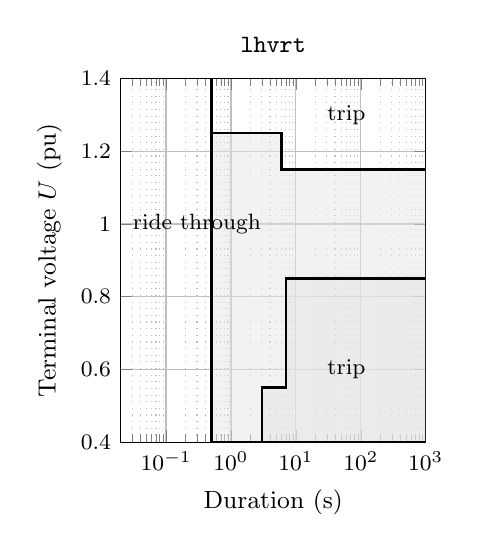
\begin{tikzpicture}
\begin{axis}[width=0.45\linewidth,height=62mm,xmode=log,xmin=0.02,xmax=1000,ymin=0.4,ymax=1.4,
  xlabel={Duration (s)},ylabel={Terminal voltage $U$ (pu)},grid=both,minor grid style={dotted},
  title={\texttt{lhvrt}},title style={font=\small},label style={font=\small},tick label style={font=\footnotesize}]
  \addplot[thick,const plot,fill=gray!20,fill opacity=0.5,draw=black] coordinates {(0.5,1.4) (0.5,1.25) (6,1.15) (1000,1.15) (1000,1.4)} \closedcycle;
  \addplot[thick,const plot,fill=gray!20,fill opacity=0.5,draw=black] coordinates {(3,0.4) (3,0.55) (7,0.85) (1000,0.85) (1000,0.4)} \closedcycle;
  \node[font=\footnotesize] at (axis cs:60,1.3) {trip};
  \node[font=\footnotesize] at (axis cs:60,0.6) {trip};
  \node[font=\footnotesize] at (axis cs:0.3,1.0) {ride through};
\end{axis}
\end{tikzpicture}\hfill
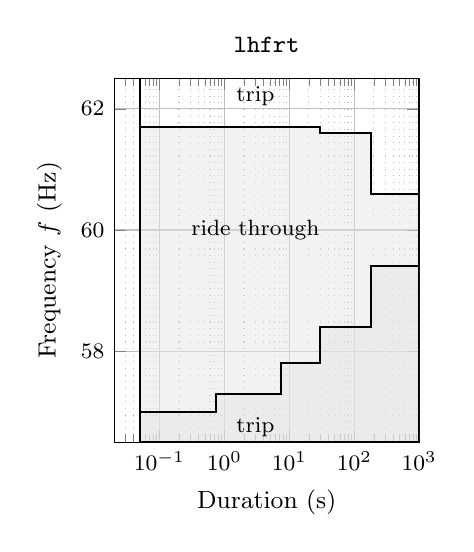
\begin{tikzpicture}
\begin{axis}[width=0.45\linewidth,height=62mm,xmode=log,xmin=0.02,xmax=1000,ymin=56.5,ymax=62.5,
  xlabel={Duration (s)},ylabel={Frequency $f$ (Hz)},grid=both,minor grid style={dotted},
  title={\texttt{lhfrt}},title style={font=\small},label style={font=\small},tick label style={font=\footnotesize}]
  \addplot[thick,const plot,fill=gray!20,fill opacity=0.5,draw=black] coordinates {(0.05,62.5) (0.05,61.7) (30,61.6) (180,60.6) (1000,60.6) (1000,62.5)} \closedcycle;
  \addplot[thick,const plot,fill=gray!20,fill opacity=0.5,draw=black] coordinates {(0.05,56.5) (0.05,57.0) (0.75,57.3) (7.5,57.8) (30,58.4) (180,59.4) (1000,59.4) (1000,56.5)} \closedcycle;
  \node[font=\footnotesize] at (axis cs:3,62.2) {trip};
  \node[font=\footnotesize] at (axis cs:3,56.75) {trip};
  \node[font=\footnotesize] at (axis cs:3,60) {ride through};
\end{axis}
\end{tikzpicture}
\caption{Must-trip regions (shaded) defined by the \texttt{lhvrt} and \texttt{lhfrt} settings. A unit trips once the terminal quantity has remained inside a shaded region for the duration on the abscissa.}
\label{fig:rt}
\end{figure}

\section{Observations}
\label{sec:obs}

A few points stand out from the two files and may deserve a check with the data
provider before the model is used in studies.

The gross scheduled dispatch of 447\,MW against 136\,MW of auxiliary load yields
about 311\,MW net at the generator buses, well below the 400\,MW in the case title,
so the title figure refers to nameplate rather than to the dispatch in this case.
Bus~22 hosts one Turboden and one Baker Hughes machine, so the two units on that bus
have different dynamics even though they share a GSU. The GSU between buses~21
and~23 carries circuit identifier~11 where the other three carry~1, which is
harmless but inconsistent. The \texttt{pss2a} gain $K_{S2} = 0.501$ implies a design
inertia of $H = 2.0$\,s rather than the modelled 1.49--1.50\,s. Finally, the POI is
modelled as an infinite bus (\texttt{gencls}, $H = 999$\,s) and the Phase~1 tie is
represented only by its line to bus~2 with no equipment behind it, so the case as
delivered is a plant-only model intended to be merged into a full-system case for
interconnection studies.

\section{References}
\label{sec:refs}
\begin{enumerate}[label={[\arabic*]}]
  \item Fervo Energy, \emph{Cape Station Phase 2 --- PSLF power-flow network case},
        filed with this report as \path{references/ModelEPC_Fervo_Cape Station_Ph2_v24_2026.09.05.epc},
        PSLF version 24.3.0, exported September 5, 2026.
  \item Fervo Energy, \emph{Cape Station Phase 2 --- PSLF dynamic data},
        filed with this report as \path{references/ModelDYD_Fervo_Cape Station_Ph2_2026.09.05.dyd},
        September 5, 2026.
  \item P.~Kundur, \emph{Power System Stability and Control}, McGraw-Hill, 1994,
        chapter~12 (small-signal stability) and section~17.2 (power system
        stabilizers).
  \item IEEE Std~421.5-2016, \emph{IEEE Recommended Practice for Excitation System
        Models for Power System Stability Studies}, IEEE Power and Energy Society,
        2016. Type AC8B excitation system and type PSS2A stabilizer.
\end{enumerate}


\end{document}
